%group_pres.tex

\documentclass{beamer}
\mode<presentation>
\usetheme{default}

\usepackage{graphicx}                  %use package for diagram 
\usepackage{amsmath}                   %use package for implies symbol
\usepackage{amsfonts}		       %use package for numbet sets
\usepackage{bm}                        %use package for bolds in math mode
\usepackage{tikz}                      %use package for diagram drawings
\usepackage{algpseudocode}             %use package for pseudocode
\usepackage{algorithm}                 %use package for pseudocode
\usepackage{caption}                   %use package for multiple figures
\usepackage{subcaption}                %use package for multiple figures
\usepackage{color}                     %use package for code listings
\usepackage{listings}                  %use package for c++ code in appendix
\usepackage[utf8]{inputenc}            %use package for colours in code
\usepackage{array}                     %use package for centering table contents
\usepackage{microtype}		       %use package for small typographical changes

%define colours for code listings
\definecolor{codegreen}{rgb}{0,0.6,0}
\definecolor{codegray}{rgb}{0.5,0.5,0.5}
\definecolor{codepurple}{rgb}{0.58,0,0.82}
\definecolor{backcolour}{rgb}{0.95,0.95,0.92}

%define a style for the listings
\lstdefinestyle{mystyle}{
    backgroundcolor=\color{backcolour},
    commentstyle=\color{codegreen},
    keywordstyle=\color{magenta},
    numberstyle=\tiny\color{codegray},
    stringstyle=\color{codepurple},
    basicstyle=\footnotesize,
    breakatwhitespace=false,
    breaklines=true,
    captionpos=b,
    keepspaces=true,
    numbers=left,
    numbersep=5pt,
    showspaces=false,
    showstringspaces=false,
    showtabs=false,
    tabsize=2,
    language=C++
}

%set style of listing to that defined above
\lstset{style=mystyle}

%set style of footnotes
\renewcommand{\thefootnote}{\roman{footnote}}

%define command shortcuts
\newcommand{\be}{\begin{equation}}
\newcommand{\ee}{\end{equation}}

%use tikz library for shapes
\usetikzlibrary{shapes.geometric, arrows}

%define block styles in tikz
\tikzstyle{startstop} = [rectangle, rounded corners, minimum width=3cm, minimum height=1cm, text centered, draw=black, fill=red!30]
\tikzstyle{io} = [trapezium, trapezium left angle=70, trapezium right angle=110, minimum width=3cm, minimum height=1cm, text centered, draw=black, fill=blue!30]
\tikzstyle{process} = [rectangle, minimum width=3cm, minimum height=1cm, text centered, draw=black, fill=orange!30]
\tikzstyle{decision} = [diamond, minimum width=3cm, minimum height=1cm, text centered, draw=black, fill=green!30]
\tikzstyle{arrow} = [thick,->,>=stealth]

%set graphics path
\graphicspath{{/home/danmfr/p3t/laplace/images/}}

\title{$3^{rd}$ Year Theoretical Physics Group Project}
\subtitle{On numerical approximations to solutions of Laplace's equation for different boundary conditions}
\author{S. Brown, F. Hayes, L. Heikkil{\"a}, D. Richardson\\
        School of Physics and Astronomy,\\
        University of Glasgow,\\
        Glasgow, United Kingdom}
\date{\today}

%layout page at start of new section
\AtBeginSection[]
{
  \begin{frame}<beamer>
    \frametitle{Layout}
    \tableofcontents[currentsection,currentsubsection]
  \end{frame}
}

\begin{document} %start of document

\begin{frame} 
\titlepage
\end{frame}

\begin{frame}
\tableofcontents
\end{frame}

\section{Overview}
\begin{frame}{Overview}
Aims:

This discussion of the Laplace equation occurs within the framework of EM but can
be generalised to other physical phenomena where the equation occurs:
thermodynamics, fluid mechanics, astronomy.
\end{frame}

\section{Introduction}
\subsection{Derivation of Laplace's Equation}

\begin{frame}{Derivation of Laplace's Equation in Electromagnetism}
Consider two of Maxwell's equations, Gauss' Law and Faraday's Law:
%
\be
\nabla \cdot \bm{E} = \frac{\rho}{\epsilon_0} \qquad \nabla \times \bm{E} = -\frac{\partial \bm{B}}{\partial t}
\ee

In static free space:
\begin{itemize}
 \item $\bm{B}$ is unchanging $\implies$ $\bm{E}$ is irrotational $\implies \bm{E} = -\nabla \phi$
 \item $\rho=0$ $\implies \bm{E}$ is solenoidal $\implies \nabla^2 \phi = 0$.
\end{itemize}

This is Laplace's equation.
\begin{itemize}
 \item $2^{nd}$ order PDE that can be solved to find $\phi$ and hence $\bm{E}$
 \item $\bm{E}$ allows equation of motion of test particles to be found (Lorentz force)
\end{itemize}
\end{frame}

\subsection{Physical Systems}

\begin{frame}{Electrostatic Systems}
\begin{figure}
\centering
\begin{subfigure}[b]{0.45\textwidth}
	\begin{tikzpicture}
	\draw (0,0) -- (0,2.5) node[above, font=\footnotesize] {$\phi = V$}; 
	\draw (4.2,0) -- (4.2,2.5) node[above, font=\footnotesize] {$\phi = -V$}; 
	\draw (2.1,1.25) circle (0.5cm) node[below, font=\footnotesize, yshift=-0.4cm] {GND};
	\draw[dashed] (2.1,1.25) -- (2.5,1.55) node[pos=0.2, above, font=\footnotesize] {$R$};
	\end{tikzpicture}
	\caption{System A}
\end{subfigure}
\hfill
\begin{subfigure}[b]{0.45\textwidth}
	\begin{tikzpicture}
	\draw (0,0) -- (4,0) node[right, font=\footnotesize] {$\phi = V$}; 
	\draw (0,2.5) -- (4,2.5) node[pos=0.25, above, font=\footnotesize] {GND} node[pos=0.5, above, font=\footnotesize] {GND} node[pos=0.75,above, font=\footnotesize] {GND};
	\draw (0.8,2.5) rectangle (1.2,2.375);
	\draw (1.8,2.5) rectangle (2.2,2.375);
	\draw (2.8,2.5) rectangle (3.2,2.375);
	\end{tikzpicture}
	\caption{System C}
\end{subfigure}
\caption{Cross-sectional diagram of two electrostatic systems}
\end{figure}

System A can be solved analytically
\begin{itemize}
\item use it to find best method to numerically solve more complex systems like C, that
do not have analytical solutions.
\end{itemize}
\end{frame}

\subsection{Analytical Solution of System A}

\begin{frame}{General Analytical Solution}
\begin{figure}
\centering
	\begin{tikzpicture}
	\draw (0,0) -- (0,2.5) node[above, font=\footnotesize] {$\phi = V$}; 
	\draw (4.2,0) -- (4.2,2.5) node[above, font=\footnotesize] {$\phi = -V$}; 
	\draw (2.1,1.25) circle (0.5cm) node[below, font=\footnotesize, yshift=-0.4cm] {GND};
	\draw[dashed] (2.1,1.25) -- (2.5,1.55) node[pos=0.2, above, font=\footnotesize,] {$R$};
	\end{tikzpicture}
	\caption{System A}
\end{figure}

To exploit the symmetry of the system we find the general solution of $\nabla^2 \phi=0$
in plane polar co-ordinates: 
%
\be
\frac{1}{r}\frac{\partial}{\partial r}(r \frac{\partial \phi}{\partial r}) + \frac{1}{r^2}\frac{\partial ^2 \phi}{\partial \theta^2} = 0 
\ee

Separate variables, $\phi(r,\theta)=f(r)g(\theta)$, say.

Substitution gives
%
\be
\frac{r}{f(r)}\frac{d}{dr}(r \frac{df(r)}{dr}) =- \frac{1}{g(\theta)}\frac{d^2 g(\theta)}{d \theta^2}
\ee

\end{frame}

\begin{frame}{General Analytical Solution cont.}
We had that supposing $\phi(r,\theta)=f(r)g(\theta)$ gave:
%
\be
\frac{r}{f(r)}\frac{d}{dr}(r \frac{df(r)}{dr}) =- \frac{1}{g(\theta)}\frac{d^2 g(\theta)}{d \theta^2}
\ee
%
Left-hand side is solely a function of $r$; right-hand side of $\theta$ 
\begin{itemize}
\item both sides must be constant, so set equal to $k^2$ say, for some $k \in \mathbb{R}$.
\end{itemize}

Produces pair of second-order ODEs:
%
\be
r\frac{d}{dr}(r \frac{df(r)}{dr}) = k^2 f(r) \quad \frac{d^2 g(\theta)}{d\theta^2} = -k^2 g(\theta)
\ee

\end{frame}

\begin{frame}{General Analytical Solution cont.}
Solutions of two ODEs:
\begin{itemize}
\item $k=0$:
\be
f(r)=\alpha_0 \ln(r) + \beta_0  \quad \text{and} \quad g(\theta)=\gamma_0 \theta +\delta_0
\ee
\item $k \neq 0$:
\be
f(r)=\alpha_k r^k +\beta_k r^{-k} \quad \text{and} \quad g(\theta) = \gamma_k \sin(k\theta) +\delta_k \cos(k\theta)
\ee
\end{itemize}

Expect $g$: $g(\theta+2\pi)=g(\theta)$ to be single-valued so that $k \in \mathbb{Z}$.

Principle of superposition gives general solution of Laplace's equation in polar
co-ordinates:
%
\begin{multline}
\phi(r, \theta) = (\alpha_0 \ln(r) + \beta_0)(\gamma_0\theta + \delta_0) \\
                + \sum_{n=1}^{\infty}(\alpha_n r^n+\beta_n r^{-n})(\gamma_n \sin(n\theta) + \delta_n \cos(n\theta))
\end{multline}

\end{frame}

\begin{frame}{Particular Solution for System A}
To find particular solution we impose \emph{Dirichlet boundary conditions}.

We have the general solution
%
\begin{multline}
\phi(r, \theta) = (\alpha_0 \ln(r) + \beta_0)(\gamma_0\theta + \delta_0) \\
                + \sum_{n=1}^{\infty}(\alpha_n r^n+\beta_n r^{-n})(\gamma_n \sin(n\theta) + \delta_n \cos(n\theta))
\end{multline}

Conditions:
\begin{itemize}
\item $\phi$ is symmetric in $\pm\theta$ or about $\theta=0 \implies \gamma_n=0, \; \forall n$
\item $\phi$ is finite at infinity $\implies \alpha_n=0, \; \forall n$
\end{itemize}

Hence
%
\be
\phi(r, \theta) = \beta_0 + \sum_{n=1}^{\infty} \frac{\beta_n}{r^n} \cos(n\theta)
\ee
%
where the $\beta$'s absorbed other constants.
\end{frame}

\begin{frame}{Particular Solution for System A cont.}
We have
%
\be
\label{eq:sum}
\phi(r, \theta) = \beta_0 + \sum_{n=1}^{\infty} \frac{\beta_n}{r^n} \cos(n\theta)
\ee

As $r \rightarrow \infty$, $\phi$ is linearly decreasing between the plates:
%
\be
\phi \rightarrow -\frac{Vx}{d}=-\frac{Vr}{d}\cos(\theta)
\ee.

Thus, $\beta_0=-\frac{Vr}{d}\cos(\theta)$, since the $2^{nd}$ term in eq.~\ref{eq:sum} 
vanishes.

Then,
%
\be
\phi(r, \theta) = -\frac{Vr}{d}\cos(\theta) + \sum_{n=1}^{\infty} \frac{\beta_n}{r^n} \cos(n\theta)
\ee
%
or,
%
\be
\phi(r, \theta) = (\frac{\beta_1}{r}-\frac{Vr}{d})\cos(\theta) + \sum_{n=2}^{\infty} \frac{\beta_n}{r^n} \cos(n\theta)
\ee

\end{frame}

\begin{frame}{Particular Solution for System A cont.}
We have
%
\be
\phi(r, \theta) = (\frac{\beta_1}{r}-\frac{Vr}{d})\cos(\theta) + \sum_{n=2}^{\infty} \frac{\beta_n}{r^n} \cos(n\theta)
\ee

Expect continuity of $\phi$ at the surface of the cylinder:
%
\be
\phi(r=R,\theta) = 0 \implies \beta_1=\frac{VR^2}{d} \quad
\text{and} \quad \beta_{n \geq 2} = 0
\ee
%
since the set $\{\cos(n \theta)\}$ are linearly independent functions.

Final solution is:
%
\be
\phi(r, \theta) = \frac{V}{d}(\frac{R^2}{r}-r)\cos(\theta)
\ee
for $r>R$ and $0$ otherwise.

\end{frame}

\begin{frame}{Analytical Solution}

\begin{figure}[h!]
\begin{center}
\includegraphics[scale=0.8]{analytic.pdf}
\caption{Analytic solution with $V=1$, $R=15$}
\end{center}
\end{figure}

\end{frame}

\section{Numerical Methods}
\begin{frame}{Necessity of numerical methods}
System A is a very idealised system, that is not realisable in the real world
\begin{itemize}
\item plates cannot be infinite in extent
\end{itemize}

For real world systems is it difficult, and often impossible, to express boundary
conditions in a manner that is algebraically usable, and thus impossible to find a
particular analytical solution to Laplace's equation.
\begin{itemize}
\item One must solve Laplace's equation numerically.
\end{itemize}

One such way is Finite Difference Methods.
\end{frame}

\subsection{Finite Difference Methods}

\begin{frame}{Finite Difference Methods}
We use the definition of the derivative, for a function $f(t)$ say, and approximate as
%
\be
\frac{df}{dt} = \lim_{\Delta t\to 0}\frac{f(t+\Delta t) - f(t)}{\Delta t} \approx \frac{f(t+\Delta t) - f(t)}{\Delta t}
\ee
%
where $\Delta t$ is assumed to be small enough that the approximation is good.

We can then approximate the second derivative similarly:
%
\begin{align}
\frac{d^2 f}{dt^2} &\approx \frac{f'(t+\Delta t) - f'(t)}{\Delta t} \\
		   &= \frac{\frac{f(t+\Delta t) - f(t)}{\Delta t} - \frac{f(t) - f(t-\Delta t)}{\Delta t}}{\Delta t} \\
\frac{d^2 f}{dt^2} &\approx  \frac{f(t+\Delta t) - 2f(t) + f(t-\Delta t)}{\Delta t^2}
\end{align}

\end{frame}

\begin{frame}{Finite Difference Methods cont.}

Define a region on which to discretise Laplace equation, 
%
\be
\{(x,y)|\:0<x<L,0<y<D\}
\ee

Create a grid of points at which to solve the equation:

\begin{figure}
\centering
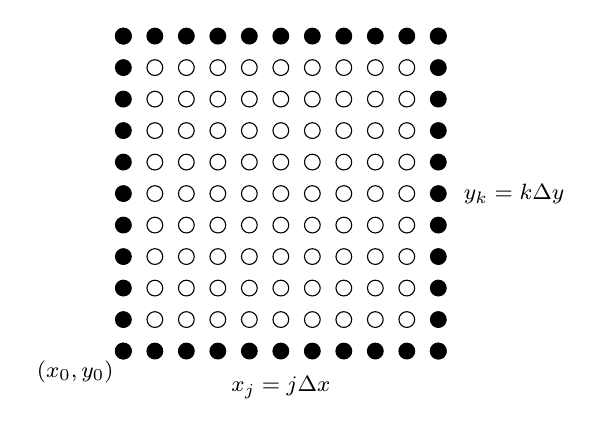
\begin{tikzpicture}

\foreach \x in {0,...,10}
{
\draw[fill=black] (0.4*\x,0) circle (0.1cm);
\draw[fill=black] (0.4*\x,4) circle (0.1cm);
}

\foreach \y in {0,...,10}
{
\draw[fill=black] (0,0.4*\y) circle (0.1cm);
\draw[fill=black] (4,0.4*\y) circle (0.1cm);
}

\foreach \x in {1,...,9}
\foreach \y in {1,...,9}
{
\draw[fill=white] (0.4*\x,0.4*\y) circle (0.1cm);
}
\fill (0,0) node[below left, font=\footnotesize] {$(x_0,y_0)$};
\fill (2,0) node[below, font=\footnotesize, yshift = -0.2cm] {$x_j=j\Delta x$};
\fill (4,2) node[right, font=\footnotesize, xshift = 0.2cm] {$y_k=k\Delta y$};
\end{tikzpicture}
\caption{Diagram of grid on which we approximate the potential $\phi$. White points
are interior points that change; black points are boundary points that remain constant.}
\end{figure}

\end{frame}

\begin{frame}{Discretisation of Laplace's equation}
We write the value of $\phi$ at position $(x_j,y_k)$ on the grid as $\phi_{j,k}$.

Hence, Laplace's eqaution is discretised as
%
\be
\frac{\phi_{j+1,k}-2\phi_{j,k}+\phi_{j-1,k}}{\Delta x^2} + \frac{\phi_{j,k+1}-2\phi_{j,k}+\phi_{j,k-1}}{\Delta y^2}=0
\ee
%
where $j$ and $k$ index the $x$ and $y$ directions.

For unique separation $\Delta = \Delta x = \Delta y$, $\phi_{j,k}$ is the average of the
surrounding points:
%
\be
\phi_{j,k}= \frac{1}{4}(\phi_{j+1,k}+\phi_{j-1,k}+\phi_{j,k+1}+\phi_{j,k-1})
\ee

\end{frame}

\section{Software}

\begin{frame}{Software Package}
\end{frame}

\begin{frame}{Flowchart}
\begin{figure}
\centerline{
\includegraphics[scale=0.7]{flowchart.pdf}
}
\end{figure}
\end{frame}

\subsection{Input}
\begin{frame}{Bitmaps}
\end{frame}

\begin{frame}{Boolean Mask}
\end{frame}

\subsection{Process}

\begin{frame}{Successive Over-relaxation}
Can define an iterative scheme which uses $\phi_{j,k,n}$:
%
\be
\phi_{j,k,n+1}= (1-s)\phi_{j,k,n}+\frac{s}{4}(\phi_{j-1,k,n+1}+\phi_{j+1,k,n}+\phi_{j,k-1,n+1}+\phi_{j,k+1,n})
\ee
%
where $1<s<2$ is the \emph{relaxation parameter}.

Optimum relaxation parameter, for an $n\times n$ square grid, is:
\be
s = \frac{2}{1+\sin(\frac{\pi}{n})} \approx \frac{2}{1+\frac{\pi}{n}}
\ee

This is a more convergent numerical method than those previous, and is called 
\emph{successive over-relaxation}.
\end{frame}

\begin{frame}{Checkerboard (Red-Black) Updating}
Algorithm:
\begin{itemize}
\item denote $\phi_{j,k}$ as \emph{odd} if $j+k$ is odd, and even otherwise.
\item iterate through the grid
 \begin{itemize}
 \item update $\phi$ at each odd point (only depends on even points)
 \end{itemize}
\item re-iterate through grid
 \begin{itemize}
 \item update all even points using $\phi$ at newly updated odd points
 \end{itemize}
\end{itemize}

This is \emph{Checkerboard (Red-Black) Updating}
\begin{itemize}
\item separates system of $N$ linear equations into two coupled systems of
$\frac{N}{2}$ linear equations.
\end{itemize}

Advantages:
\begin{itemize}
\item more convergent method than those outlined previously
\item can have successive over-relaxation added
\item employ parallel processing
\end{itemize}

\end{frame}

\begin{frame}{Checkerboard (Red-Black) Updating cont.}
\begin{figure}[h!]
\begin{center}
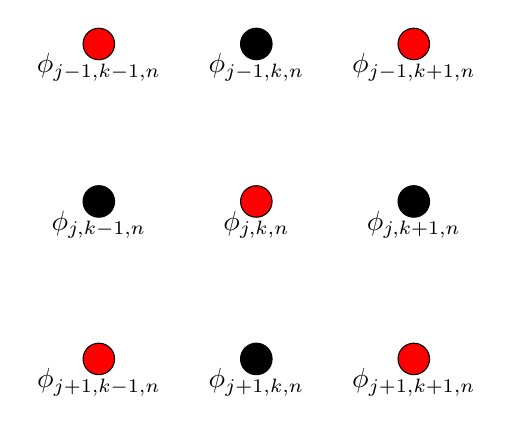
\begin{tikzpicture}
\draw[fill=red] (0,0) circle (0.2cm) node[below] {$\phi_{j+1,k-1,n}$};
\draw[fill=black] (2,0) circle (0.2cm) node[below] {$\phi_{j+1,k,n}$};
\draw[fill=red] (4,0) circle (0.2cm) node[below] {$\phi_{j+1,k+1,n}$};
\draw[fill=black] (0,2) circle (0.2cm) node[below] {$\phi_{j,k-1,n}$};
\draw[fill=red] (2,2) circle (0.2cm) node[below] {$\phi_{j,k,n}$};
\draw[fill=black] (4,2) circle (0.2cm) node[below] {$\phi_{j,k+1,n}$};
\draw[fill=red] (0,4) circle (0.2cm) node[below] {$\phi_{j-1,k-1,n}$};
\draw[fill=black] (2,4) circle (0.2cm) node[below] {$\phi_{j-1,k,n}$};
\draw[fill=red] (4,4) circle (0.2cm) node[below] {$\phi_{j-1,k+1,n}$};
\end{tikzpicture}
\end{center}
\caption{An illustration of checkerboard updating. The black points are updated first,
and then red points are calculated from the newly updated black points.}
\label{fig:checker}
\end{figure}

\end{frame}

\begin{frame}{Checkerboard (Red-Black) Updating cont.}
\begin{figure}[h!]
\begin{center}
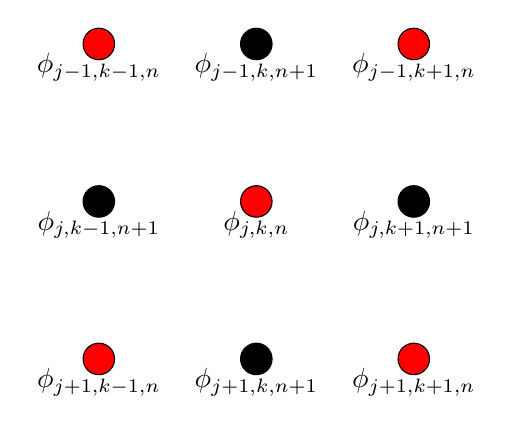
\begin{tikzpicture}
\draw[fill=red] (0,0) circle (0.2cm) node[below] {$\phi_{j+1,k-1,n}$};
\draw[fill=black] (2,0) circle (0.2cm) node[below] {$\phi_{j+1,k,n+1}$};
\draw[fill=red] (4,0) circle (0.2cm) node[below] {$\phi_{j+1,k+1,n}$};
\draw[fill=black] (0,2) circle (0.2cm) node[below] {$\phi_{j,k-1,n+1}$};
\draw[fill=red] (2,2) circle (0.2cm) node[below] {$\phi_{j,k,n}$};
\draw[fill=black] (4,2) circle (0.2cm) node[below] {$\phi_{j,k+1,n+1}$};
\draw[fill=red] (0,4) circle (0.2cm) node[below] {$\phi_{j-1,k-1,n}$};
\draw[fill=black] (2,4) circle (0.2cm) node[below] {$\phi_{j-1,k,n+1}$};
\draw[fill=red] (4,4) circle (0.2cm) node[below] {$\phi_{j-1,k+1,n}$};
\end{tikzpicture}
\end{center}
\caption{An illustration of checkerboard updating. The black points are updated first,
and then red points are calculated from the newly updated black points.}
\label{fig:checker}
\end{figure}

\end{frame}

\begin{frame}{Checkerboard (Red-Black) Updating cont.}
\begin{figure}[h!]
\begin{center}
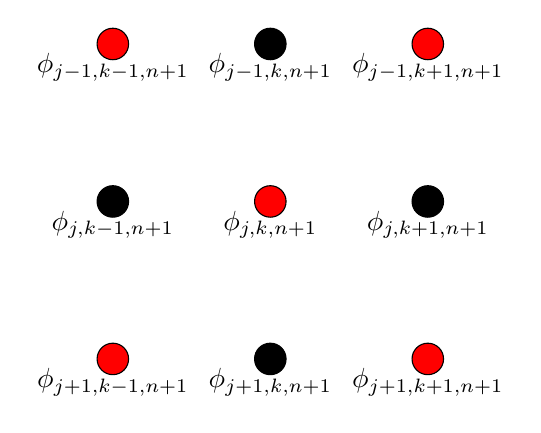
\begin{tikzpicture}
\draw[fill=red] (0,0) circle (0.2cm) node[below] {$\phi_{j+1,k-1,n+1}$};
\draw[fill=black] (2,0) circle (0.2cm) node[below] {$\phi_{j+1,k,n+1}$};
\draw[fill=red] (4,0) circle (0.2cm) node[below] {$\phi_{j+1,k+1,n+1}$};
\draw[fill=black] (0,2) circle (0.2cm) node[below] {$\phi_{j,k-1,n+1}$};
\draw[fill=red] (2,2) circle (0.2cm) node[below] {$\phi_{j,k,n+1}$};
\draw[fill=black] (4,2) circle (0.2cm) node[below] {$\phi_{j,k+1,n+1}$};
\draw[fill=red] (0,4) circle (0.2cm) node[below] {$\phi_{j-1,k-1,n+1}$};
\draw[fill=black] (2,4) circle (0.2cm) node[below] {$\phi_{j-1,k,n+1}$};
\draw[fill=red] (4,4) circle (0.2cm) node[below] {$\phi_{j-1,k+1,n+1}$};
\end{tikzpicture}
\end{center}
\caption{An illustration of checkerboard updating. The black points are updated first,
and then red points are calculated from the newly updated black points.}
\label{fig:checker}
\end{figure}

\end{frame}

\begin{frame}{Parallel Processing}

\begin{figure}[h!]
\begin{center}
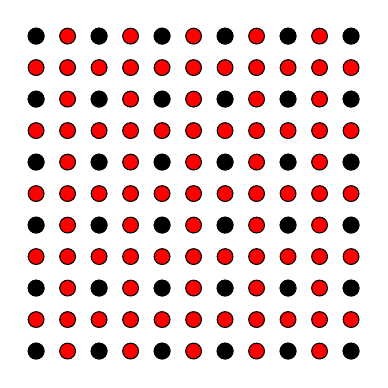
\begin{tikzpicture}
\foreach \x in {0,...,10}
{
 \foreach \y in {0,...,10}
 {
  \draw[fill=red] (0.4*\x,0.4*\y) circle (0.1cm);
 }
}

\foreach \x in {0,...,5}
{
 \foreach \y in {0,...,5}
 {
  \draw[fill=black] (0.8*\x,0.8*\y) circle (0.1cm);
 }
}

\end{tikzpicture}
\end{center}
\caption{An illustration of checkerboard updating. The black points are updated first,
and then red points are calculated from the newly updated black points.}
\label{fig:checker}
\end{figure}

\end{frame}

\begin{frame}{Convergence Locking}
If a point is deemed to converge, i.e. the absolute difference between the previous
and current potential is less than a certain desired convergence, it is set to a
boundary in the boolean mask and ignored during a pass over the grid.

When every point is locked the program is stopped, and results outputted.
\end{frame}

\begin{frame}{Convergence Locking Cont.}
\begin{figure}
\centering
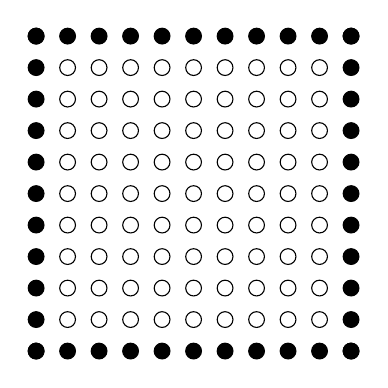
\begin{tikzpicture}

\foreach \x in {0,...,10}
{
\draw[fill=black] (0.4*\x,0) circle (0.1cm);
\draw[fill=black] (0.4*\x,4) circle (0.1cm);
}

\foreach \y in {0,...,10}
{
\draw[fill=black] (0,0.4*\y) circle (0.1cm);
\draw[fill=black] (4,0.4*\y) circle (0.1cm);
}

\foreach \x in {1,...,9}
\foreach \y in {1,...,9}
{
\draw[fill=white] (0.4*\x,0.4*\y) circle (0.1cm);
}
\end{tikzpicture}
\caption{Diagram of grid on which we approximate the potential $\phi$. White points
are interior points that change; black points are boundary points that remain constant.}
\end{figure}

\end{frame}

\begin{frame}{Convergence Locking Cont.}
\begin{figure}
\centering
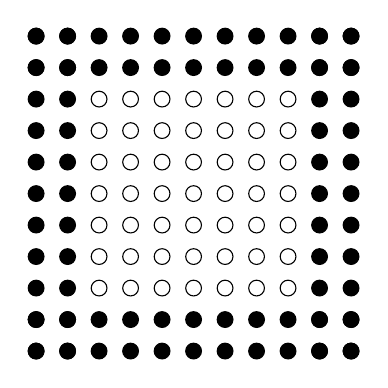
\begin{tikzpicture}

\foreach \x in {0,...,10}
{
\draw[fill=black] (0.4*\x,0) circle (0.1cm);
\draw[fill=black] (0.4*\x,0.4) circle (0.1cm);
\draw[fill=black] (0.4*\x,3.6) circle (0.1cm);
\draw[fill=black] (0.4*\x,4) circle (0.1cm);
}

\foreach \y in {0,...,10}
{
\draw[fill=black] (0,0.4*\y) circle (0.1cm);
\draw[fill=black] (0.4,0.4*\y) circle (0.1cm);
\draw[fill=black] (3.6,0.4*\y) circle (0.1cm);
\draw[fill=black] (4,0.4*\y) circle (0.1cm);
}

\foreach \x in {2,...,8}
\foreach \y in {2,...,8}
{
\draw[fill=white] (0.4*\x,0.4*\y) circle (0.1cm);
}
\end{tikzpicture}
\caption{Diagram of grid on which we approximate the potential $\phi$. White points
are interior points that change; black points are boundary points that remain constant.}
\end{figure}

\end{frame}

\begin{frame}{Convergence Locking Cont.}
\begin{figure}
\centering
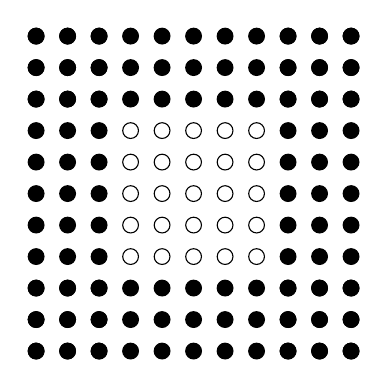
\begin{tikzpicture}

\foreach \x in {0,...,10}
{
\draw[fill=black] (0.4*\x,0) circle (0.1cm);
\draw[fill=black] (0.4*\x,0.4) circle (0.1cm);
\draw[fill=black] (0.4*\x,0.8) circle (0.1cm);
\draw[fill=black] (0.4*\x,3.2) circle (0.1cm);
\draw[fill=black] (0.4*\x,3.6) circle (0.1cm);
\draw[fill=black] (0.4*\x,4) circle (0.1cm);
}

\foreach \y in {0,...,10}
{
\draw[fill=black] (0,0.4*\y) circle (0.1cm);
\draw[fill=black] (0.4,0.4*\y) circle (0.1cm);
\draw[fill=black] (0.8,0.4*\y) circle (0.1cm);
\draw[fill=black] (3.2,0.4*\y) circle (0.1cm);
\draw[fill=black] (3.6,0.4*\y) circle (0.1cm);
\draw[fill=black] (4,0.4*\y) circle (0.1cm);
}

\foreach \x in {3,...,7}
\foreach \y in {3,...,7}
{
\draw[fill=white] (0.4*\x,0.4*\y) circle (0.1cm);
}
\end{tikzpicture}
\caption{Diagram of grid on which we approximate the potential $\phi$. White points
are interior points that change; black points are boundary points that remain constant.}
\end{figure}

\end{frame}

\begin{frame}{Convergence Locking Cont.}
\begin{figure}
\centering
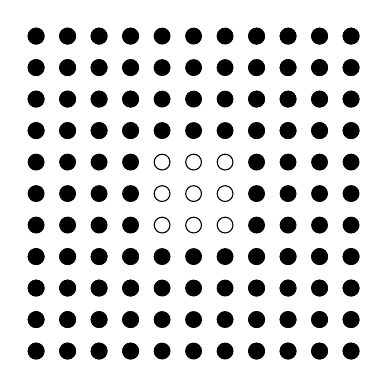
\begin{tikzpicture}

\foreach \x in {0,...,10}
{
\draw[fill=black] (0.4*\x,0) circle (0.1cm);
\draw[fill=black] (0.4*\x,0.4) circle (0.1cm);
\draw[fill=black] (0.4*\x,0.8) circle (0.1cm);
\draw[fill=black] (0.4*\x,1.2) circle (0.1cm);
\draw[fill=black] (0.4*\x,2.8) circle (0.1cm);
\draw[fill=black] (0.4*\x,3.2) circle (0.1cm);
\draw[fill=black] (0.4*\x,3.6) circle (0.1cm);
\draw[fill=black] (0.4*\x,4) circle (0.1cm);
}

\foreach \y in {0,...,10}
{
\draw[fill=black] (0,0.4*\y) circle (0.1cm);
\draw[fill=black] (0.4,0.4*\y) circle (0.1cm);
\draw[fill=black] (0.8,0.4*\y) circle (0.1cm);
\draw[fill=black] (1.2,0.4*\y) circle (0.1cm);
\draw[fill=black] (2.8,0.4*\y) circle (0.1cm);
\draw[fill=black] (3.2,0.4*\y) circle (0.1cm);
\draw[fill=black] (3.6,0.4*\y) circle (0.1cm);
\draw[fill=black] (4,0.4*\y) circle (0.1cm);
}

\foreach \x in {4,...,6}
\foreach \y in {4,...,6}
{
\draw[fill=white] (0.4*\x,0.4*\y) circle (0.1cm);
}
\end{tikzpicture}
\caption{Diagram of grid on which we approximate the potential $\phi$. White points
are interior points that change; black points are boundary points that remain constant.}
\end{figure}

\end{frame}

\begin{frame}{Convergence Locking Cont.}
\begin{figure}
\centering
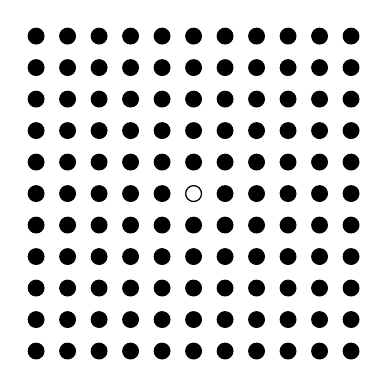
\begin{tikzpicture}

\foreach \x in {0,...,10}
{
 \foreach \y in {0,...,10}
 {
  \draw[fill=black] (0.4*\x,0.4*\y) circle (0.1cm);
 }
}

\draw[fill=white] (2,2) circle (0.1cm);

\end{tikzpicture}
\caption{Diagram of grid on which we approximate the potential $\phi$. White points
are interior points that change; black points are boundary points that remain constant.}
\end{figure}

\end{frame}

\begin{frame}{Convergence Locking Cont.}
\begin{figure}
\centering

\begin{tikzpicture}

\foreach \x in {0,...,10}
{
 \foreach \y in {0,...,10}
 {
  \draw[fill=black] (0.4*\x,0.4*\y) circle (0.1cm);
 }
}
\end{tikzpicture}
\caption{Diagram of grid on which we approximate the potential $\phi$. White points
are interior points that change; black points are boundary points that remain constant.}
\end{figure}

\end{frame}

\section{Results}

\begin{frame}{Results}
\end{frame}

\section{Analysis}
\begin{frame}{Analysis}
\end{frame}

\section{Conclusion}

\begin{frame}{Conclusion}
Further Work:
\begin{itemize}
\item Poisson's equation
\item Boundary conditions that vary with position
\end{itemize}

Alternative methods:
\begin{itemize}
\item Multigrid methods
\item Fast Fourier Transform
\item Nine-point stenciling
\end{itemize}

\end{frame}

\begin{frame}
\titlepage
\end{frame}

\end{document} %end of document
